\documentclass[titlepage=firstiscover, captions=tableheading, bibliography=totoc]{scrartcl}
\usepackage[autostyle=true,german=quotes]{csquotes}
\usepackage{scrhack}
\usepackage{caption}
\usepackage[aux]{rerunfilecheck}
\usepackage{subcaption}        
\usepackage{fontspec}
\usepackage[dvips]{graphicx}
\usepackage{floatflt,epsfig} 
    
\usepackage{polyglossia}
\setmainlanguage{german}

\usepackage[unicode]{hyperref}
\usepackage{bookmark}
\title{V27\\ Der Helium-Neon-Laser}
\author{
Miriam Simm\\
\texorpdfstring{\href{mailto:miriam.simm@tu-dortmund.de}{miriam.simm@tu-dortmund.de}\and}{,}
Katrin Bolsmann\\
\texorpdfstring{\href{mailto:katrin.bolsmann@tu-dortmund.de}{katrin.bolsmann@tu-dortmund.de}}{}
}
\date{Durchführung: 15.06.2020 \\ Abgabe: -.06.2020}
\usepackage{amsmath} 
\usepackage{amssymb} 
\usepackage{mathtools}
\usepackage[
    math-style=ISO,
    bold-style=ISO,
    sans-style=italic,
    nabla=upright,
    partial=upright,
]{unicode-math}
    
\setmathfont{Latin Modern Math}

\usepackage[
  locale=DE,
  separate-uncertainty=true, 
  per-mode=symbol-or-fraction,
]{siunitx}

\usepackage{multicol}
\setlength{\columnsep}{1pt} %space between columns 

\usepackage{booktabs}
\usepackage[x11names, table]{xcolor}
\usepackage{graphicx}
\usepackage{grffile}
\usepackage{xfrac}
\usepackage{xcolor}

\usepackage{float}
\floatplacement{figure}{h}
\floatplacement{table}{h}
\usepackage[
  section,
  below,
]{placeins}

\usepackage{expl3}
\usepackage{xparse}
\ExplSyntaxOn
\NewDocumentCommand \E {} {\symup{e}}
\ExplSyntaxOff

% Literaturverzeichnis
\usepackage[
  backend=biber,
]{biblatex}
% Quellendatenbank
\addbibresource{literatur.bib}

\usepackage[
  version=4,
  math-greek=default,
  text-greek=default,
]{mhchem}
 

\raggedcolumns

\begin{document}

\maketitle
\section{Zielsetzung}
Ziel des Versuchs ist die Bestimmung der effektiven Masse der Leitungselektronen im n-dotiertem Galliumarsenid 
mithilfe des Faraday-Effekts.

\section{Theorie}
\subsection{Bandstruktur von Halbleitern}
In kristallinen Festkörpern befinden sich die Atome in einem periodischen Gitterpotential. Jedes Elektron eines einzelnen
Atoms hat ein diskretes Energieniveau, das mit den Energieniveaus der Nachbarelektronen überlappt, wodurch eine
Struktur aus Bändern und Bandlücken entsteht. Innerhalb eines Bandes können sich die Elektronen frei bewegen, sofern nicht alle 
Zustände darin besetzt sind. 
Für die Leitfähigkeit von Festkörpern sind das Leitungs- und Valenzband wichtig.
Am absoluten Nullpunkt bei $T = 0 \si{\kelvin}$ ist das Valenzband das höchst besetzte Energieband. 
Oberhalb des Valenzbandes liegt das Leitungsband, das bei Isolatoren und Halbleitern durch eine Bandlücke vom 
Valenzband getrennt ist. Befinden sich Elektronen im Leitungsband wird das Material elektrisch leitfähig.
Bei Metallen überlappen Valenzband und Leitungsband, was ihre Leitfähigkeit erklärt.
In Abbildung \ref{fig:tfig1} ist diese Bandstruktur schematisch dargestellt.
\FloatBarrier
\begin{figure}[h]
    \centering
    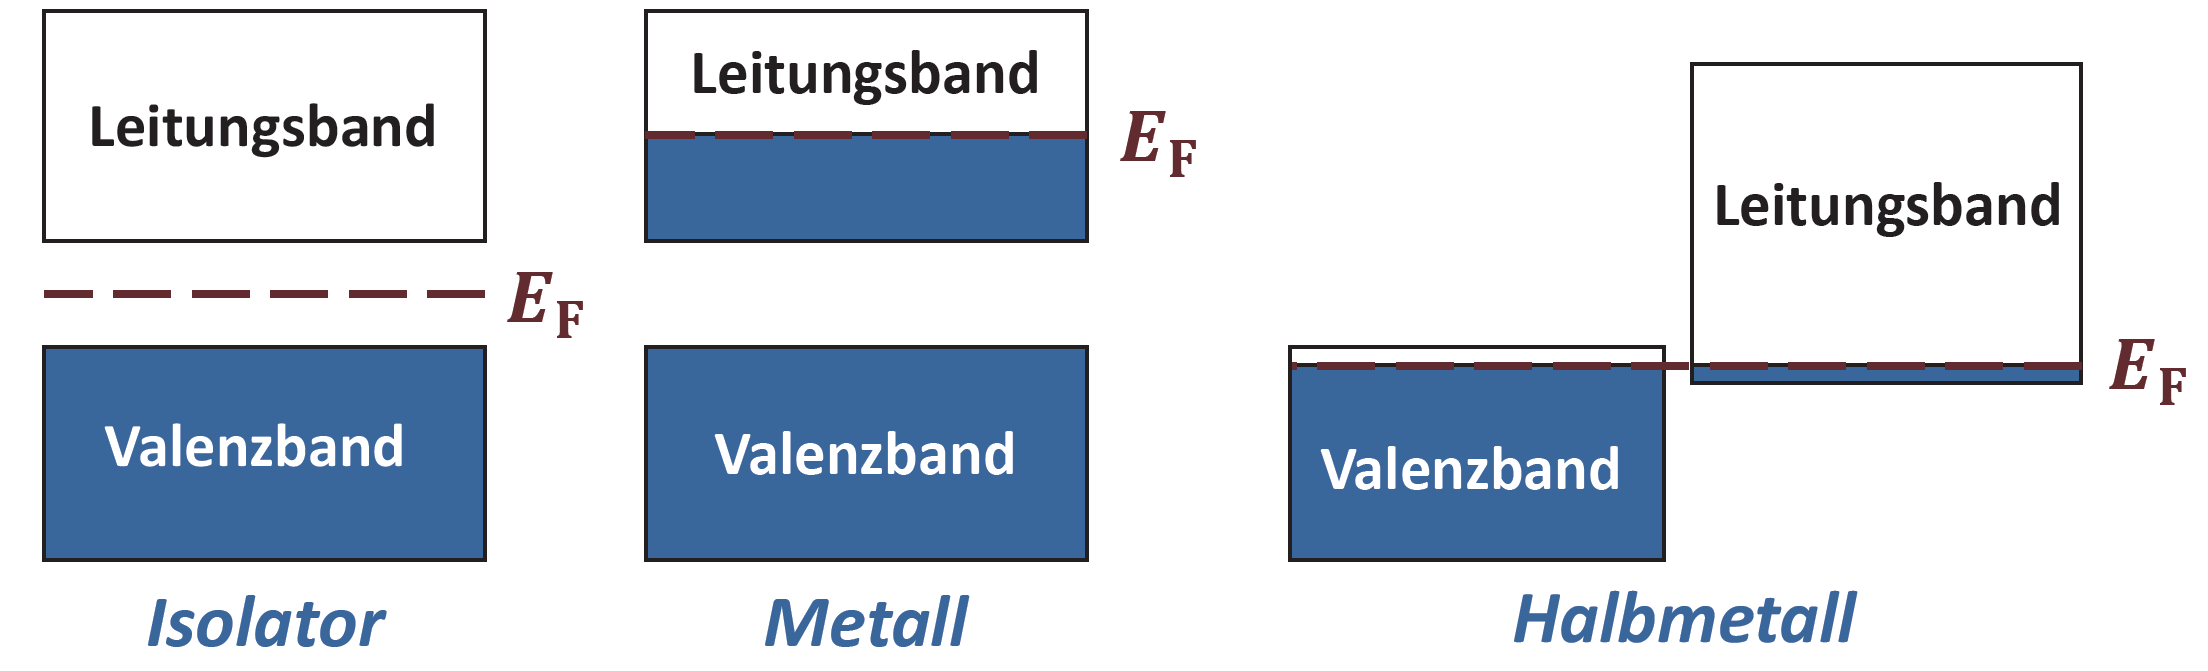
\includegraphics[width=0.9\textwidth]{band.png}
    \caption{Bandstrukur von Isolatoren, Metallen und Halbmetallen. $E_F$ bezeichnet jeweils die Fermienergie \cite[346]{quelle01}.}
    \label{fig:tfig1}
\end{figure}
\FloatBarrier
\noindent
Halbleiter sind daher am absoluten Nullpunkt nicht elektrisch leitfähig. Da die Bandlücke zwischen Leitungsband und 
Valenzband jedoch nur sehr klein ist, kann sie bei Temperaturen größer als $T = 0 \si{\kelvin}$ leicht überwunden werden. Dabei wird ein 
Elektron durch die thermische Anregung vom Leitungsband ins Valenzband angeregt und hinterlässt ein Loch im Valenzband. 
Bei Raumtemperatur haben Halbleiter daher eine geringe intrinsische Leitfähigkeit. 

Neben der Erhöhung der Temperatur kann die Leitfähigkeit eines Halbleiters auch durch Dotierung erhöht werden. Dazu 
werden Fremdatome mit anderer Wertigkeit als die Atome des Halbleiters in den Halbleiter eingebracht, wodurch die 
Ladungsträgerdichte erhöht wird. Unterschieden wird dabei zwischen n-Dotierung und p-Dotierung.
N-Dotierung bezeichnet das Einbringen von Fremdatomen mit jeweils einem Überschusselektron in den Festkörper. Diese Atome 
werden als Donatoren bezeichnet, und die Energie der Donatorelektronen liegt knapp unterhalb der Leitungsbandkante. Das Überschusselektron 
kann dann leicht ins Leitungsband angeregt werden, wodurch sich die Leitfähigkeit erhöht. 
Bei p-Dotierung wird ein Fremdatom eingebracht, das ein Elektron weniger als die Atome des Festkörpers hat. Dieses Akzeptoratom
führt zu einem zusätzlichen Loch innerhalb des Valenzbandes, das dann von anderen Valenzbandelektronen besetzt werden kann.

\subsection{Effektive Masse}
Um die Bewegung von Elektronen in einem Festkörper beschreiben zu können, wird das Konzept der effektiven Masse eingeführt.
Elektronen in einem Festkörper bewegen sich quasifrei. Wird ihre Masse durch eine effektive Masse ersetzt, die den 
Einfluss des periodischen Potentials des Gitters berücksichtigt, können sie als freie Teilchen betrachtet werden und 
ihre Bewegungsgleichung vereinfacht sich. Dazu wird $\varepsilon(\vec{k})$ bis zur zweiten Ordnung in eine
Taylorreihe um $k = 0$ entwicklelt, folgt für die effektive Masse $m^{*}$
\begin{equation*}
    m^{*}_i = \frac{\hbar^2}{\left[\frac{\partial^2 \varepsilon}{\partial k_i^2}\right]_{k = 0}} \, 
\end{equation*}
mit $i = x, y, z$.

\subsection{Faraday-Rotation}
Liegt an einem transpartenten Medium ein Magnetfeld an, so dreht
sich die Polarisationsebene einer linear polarisierten Welle beim Durchgang durch das Medium, sofern das Magnetfeld
parallel zur Ausbreitungsrichtung der Welle liegt. Dieser magnetooptische Effekt ist die Faraday-Rotation.

Eine linear polarisierte Welle kann als Überlagerung zweier zirkular polarisierter Wellen mit gleicher Frequenz
und entgegengesetzer Ausbreitungsrichtung betrachtet werden. Im Material sind dann die Brechungsindizes $n_\text{links}$ 
und $n_\text{rechts}$ unterschiedlich, weswegen sich auch die Wellenlängen unterscheiden.
\FloatBarrier
\begin{figure}[h]
    \centering
    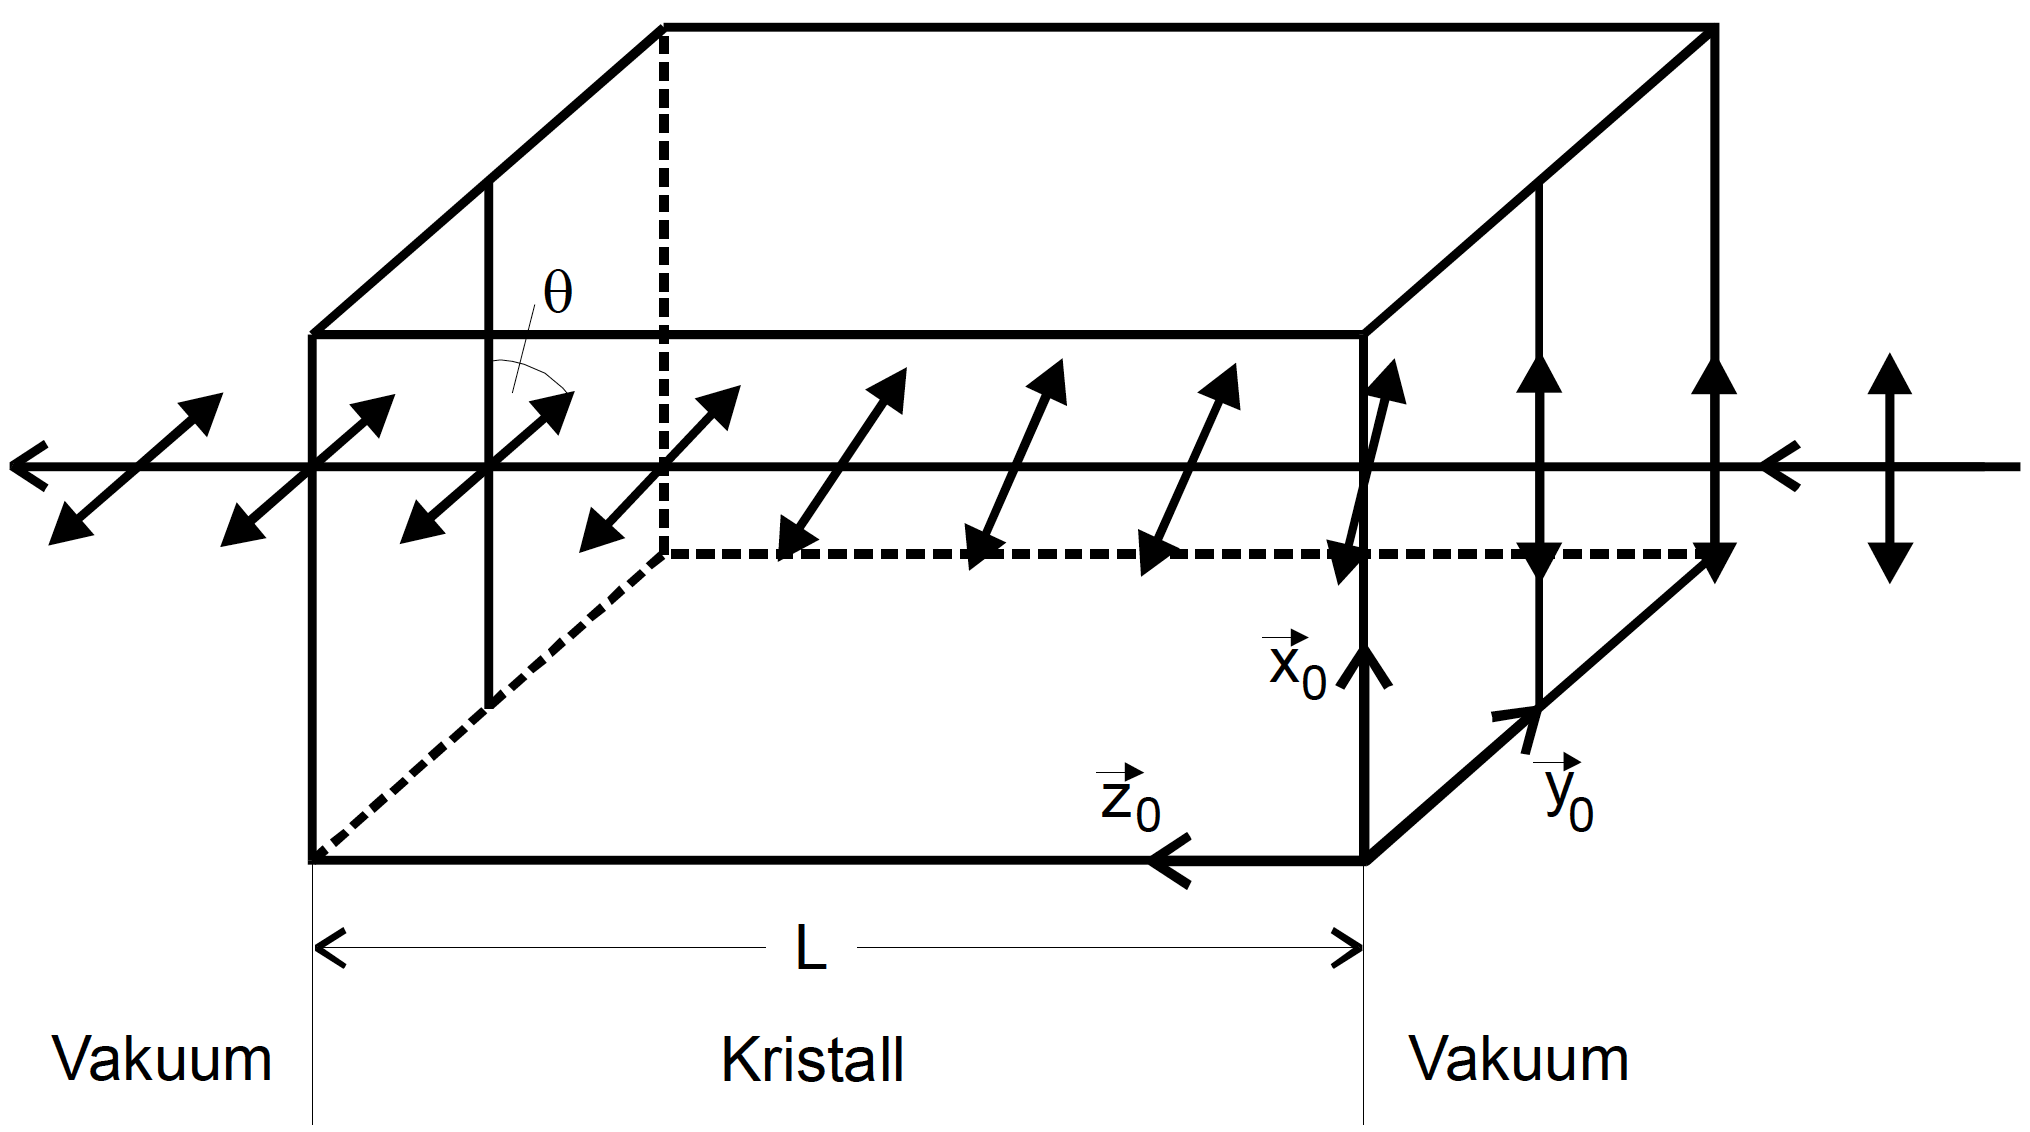
\includegraphics[width=0.9\textwidth]{rotation.png}
    \caption{Effekt der Faraday-Rotation: Drehung der Polarisationsebene eine elektromagnetischen Welle beim Durchgang durch ein Medium mit parallel zur Ausbreitungsrichtung angelegtem Magnetfeld \cite{quelle02}.}
    \label{fig:tfig2}
\end{figure}
\FloatBarrier
\noindent
Die linerar polarisierte Welle $E(z)$ wird nun in eine rechts- und linkszirkular polarisierte Welle mit Ausbreitung in 
$\vec{z}$-Richtung zerlegt
\begin{equation*}
    E(z) = \frac{E_\text{R}\left(z\right) + E_\text{L}\left(z\right)}{2} \, ,
\end{equation*}
sodass für Wellenzahlen $k_R \neq k_L$ für die Anteile gilt
\begin{align*}
    E_R (z) = \left(E_0 \vec{x_0} - i E_0 \vec{y_0}\right) \text{e}^{i k_R z} && E_L (z) = \left(E_0 \vec{x_0} + i E_0 \vec{y_0}\right) \text{e}^{i k_L z} \, .
\end{align*}
Beim Einfall in das Medium bei $z = 0$ ist die Polatisation der Welle dann parallel zur $\vec{x}$-Richtung mit $E(0) = E_0 \vec{x_0}$.
Mit einigen Umformungen folgt für den Drehwinkel
\begin{equation*}
    \theta = \frac{L \omega}{2} \left(\frac{1}{v_{Ph_R}} - \frac{1}{v_{Ph_L}}\right) \, ,
\end{equation*}
wobei $v_{Ph}$ die Phasengeschwindigkeit der rechts- bzw. linkszirkular polarisierten Welle und $L$ die Länge des Materials
bedeutet. 
%Wird der Brechungsindex $n = \frac{c}{v_{PH}}$ verwendet, vereinfacht sich diese Gleichung zu
%\begin{equation*}
%    \theta = \frac{L \omega}{2 c} \left(n_R - n_L\right)
%\end{equation*}
Grund für diesen Effekt sind induzierte elektrische Dipolmomente innerhalb des Materials. Diese entstehen durch die Atome
auf den Gitterplätzen, aber auch durch die Bandelektronen, die mit den Atomrümpfen wechselwirken. Zusammen erzeugen diese
Dipole eine makroskopische Polarisation $\vec{P}$ des Materials. Bei hinreichend kleinem elektrischen Feld gilt für die 
Polarisation der Zusammenhang
\begin{equation}
    \label{eq:Pol}
    \vec{P} = \varepsilon_0 \chi \vec{E}
\end{equation}
mit der dielektrischen Suszeptibilität $\chi$. Ist das Material isotrop ist die Suszeptibilität ein Skalar, im Allgemeinen
ist sie jedoch ein Tensor
\begin{equation*}
    \begin{pmatrix}
        P_x \\
        P_y \\
        P_z
    \end{pmatrix}
    = \varepsilon_0 \begin{pmatrix}
        \chi_{xx} & \chi_{xy} & \chi_{xz} \\
        \chi_{yx} & \chi_{yy} & \chi_{yz} \\
        \chi_{zx} & \chi_{zy} & \chi_{zz}
    \end{pmatrix}
    \begin{pmatrix}
        E_x \\
        E_y \\
        E_z 
    \end{pmatrix} \, .
\end{equation*}
Dieser Tensor ist oft symmetrisch, sodass eine Hauptachsentransformation durchgeführt werden kann. Falls im Suszeptibilitätstensor
jedoch nicht-diagonale, konjugiert komplexe Koeffizienten auftreten, ist Doppelbrechung im Material möglich.
Der Tensor hat dann die Form 
\begin{equation}
    \label{eq:tensor}
    \chi
    = \begin{pmatrix}
        \chi_{xx} & i \, \chi_{xy} & 0 \\
        - i \, \chi_{yx} & \chi_{yy} & 0 \\
        0 & 0 & \chi_{zz}
    \end{pmatrix} \, .
\end{equation}
Mit der elektromagnetischen Wellengleichung und der dielektrischen Verschiebung $\vec{D} = \varepsilon_0 \vec{E} + \vec{P}$
folgt für die Wellenzahl $k$
\begin{equation*}
    k_{\pm} = \frac{\omega}{c} \sqrt{\left(1 + \chi_{xx} \right) \pm \chi_{xy}} \, .
\end{equation*}
Daraus folgen mit $v = \frac{\omega}{k}$ zwei Phasengeschwindigkeiten
\begin{align*}
    v_{Ph_R} = \frac{c}{\sqrt{1 + \chi_{xx} + \chi_{xy}}} && v_{Ph_L} = \frac{c}{\sqrt{1 + \chi_{xx} - \chi_{xy}}} \, ,
\end{align*}
die größer bzw. kleiner als die Phasengeschwindigkeit 
\begin{equation*}
    v_{Ph} = \frac{c}{\sqrt{1 + \chi_{xx}}}
\end{equation*}
bei $\chi_{xy} = 0$ sind. Für die Feldstärkekomponenten der durchlaufenden Welle folgt dann
\begin{equation*}
    E_x = \begin{cases}
        + i E_y & \text{für} \; k_{+} \\
        - i E_y & \text{für} \; k_{-} \, ,
    \end{cases}
\end{equation*}
was zeigt, dass die linkszirkular und rechtszirkular polarisierte Welle verschiedene Phasengeschwindigkeiten haben, 
sodass die Polarisationsrichtung der Welle beim Durchgang durch das Medium gedreht wird. Der Drehwinkel $\theta$ ist dann
\begin{equation*}
    \theta = \frac{L}{2} \left(k_{x} - k_{-}\right) \, .
\end{equation*}
Da $\chi_{xy}$ klein gegen $1 + \chi_{xx}$ ist gilt dann näherungsweise
\begin{equation*}
    \theta \approx \frac{L \omega}{2 c n} \chi_{xy} \, .
\end{equation*}
\subsection{Einfluss des Magnetfeldes}
Bei optisch inaktiver Materie gilt für die Einträge des Suszeptibilitätstensors $\chi$ nun dass $\chi_{ij} = 0$ für $i \neq j$, 
sodass der Effekt der zirkularen Doppelbrechung nicht auftritt. Das ändert sich, wenn ein Magnetfeld angelegt wird. 
Ein gebundenes Elektron folgt dann der Bewegungsgleichung
\begin{equation*}
    m \frac{\text{d}^2 \vec{r}}{\text{d} t^2} + K \vec{r} = - e_0 \vec{E}(r) - e_0 \frac{\text{d} \vec{r}}{\text{d} t} \times \vec{B} \, ,
\end{equation*} 
wobei $m$ die Masse und $e_0$ die Ladung des Elektrons, $K$ eine Konstante, die die Bindung an die Umgebung beschreibt, und
$\vec{r}$ die Auslenkung aus der Ruhelage ist. Für die Feldstärke $\vec{E}$ gilt $E(t) \sim \text{e}^{- i \omega t}$ und
mit der Polarisation $\vec{P} = - N e_0 \vec{r}$ folgt
\begin{equation*}
    -m \omega^2 \vec{P} + K \vec{P} = e_0^2 N \vec{E} + i e_0 \omega \vec{P} \times \vec{B}
\end{equation*}
mit Komponenten
\begin{align}
    \label{eq:bfeld}
    \left(- m \omega ^2 + K\right) P_x &= N e_0^2 E_x + i e_0 \omega P_y B \\
    \left(- m \omega ^2 + K\right) P_y &= N e_0^2 E_y - i e_0 \omega P_x B \\
    \left(- m \omega ^2 + K\right) P_z &= N e_0^2 E_z  
\end{align}
bei einem Magnetfeld in $z$-Richtung. Weiterhin gilt für die Polarisation auch Gleichung \eqref{eq:Pol} und für eine nichttriviale 
Lösung der Gleichungen \eqref{eq:bfeld} müssen nicht-diagonale Elemente im Suszeptibilitätstensor existieren. Damit diese
Elemente unabhängig von den Feldstärkekomponenten $E_x$ und $E_y$ sind müssen sie imaginär sein, und nach der Trennung von
\eqref{eq:bfeld} in Real- und Imaginärteil hat der Suszeptibilitätstensor die gleiche Gestalt wie in Gleichung \eqref{eq:tensor}.
Mit der Tensorkompontente $\chi_{xy}$ ergibt sich der Drehwinkel dann zu
\begin{equation*}
    \theta = \frac{e_0^3}{2 \varepsilon_0 c m^2} \frac{\omega^2}{\left(- m \omega^2 + \frac{K}{m}\right)^2 - \left(\frac{e_0}{m} \omega B\right)^2} \frac{N B L}{n} \, . 
\end{equation*}
Hierbei ist $\sqrt{\frac{K}{m}}$ die Resonanzfrequenz $\omega_0$ und $\frac{B e_0}{m}$ die Zyklotronfrequenz $\omega_c$, 
die bei einem Magnetfeld $B \approx 1 \si{\tesla}$ die Größenordnung $10^{11} \si{\hertz}$ hat. Die Messfrequenz und die
Resonanzfrequenz bei Halbleitern liegt meistens im nahen Infrarotbereich, $\omega_0 = 10^{14} - 10^{15} \si{\hertz}$, 
weswegen gilt dass
\begin{equation*}
    \left(\omega_0^2 - \omega^2\right) ^2 \gg \omega^2 \omega_c^2 \, .
\end{equation*} 
Mit einer Messfrequenz, die weit unterhalb von $\omega_0$ liegt ergibt sich für den Winkel $\theta$ in Abhängigkeit von
der Wellenlänge $\lambda$
\begin{equation}
    \label{eq:Winkel2}
    \theta \left(\lambda\right) \approx \frac{2 \pi^2 e_0^3 c}{e_0 m^2} \frac{1}{\lambda^2 \omega_0^4} \frac{N B L}{n} \, .
\end{equation}
Im Grenzfall $\omega_0 \rightarrow 0$ folgt mit der effektiven Masse $m^{*}$ für quasifreie Elektronen
\begin{equation}
    \label{eq:Winkel}
    \theta_\textit{frei} = \frac{e_0^3}{8 \pi^2 e_0 c^3} \frac{\lambda^2}{\left(m^{*}\right)^2} \frac{N B}{n} \, .
\end{equation}

\section{Aufbau}
Der in diesem Versuch verwendete Aufbau ist in Abbildung \ref{fig:aufbau} dargestellt.
\FloatBarrier
\begin{figure}[h]
    \centering
    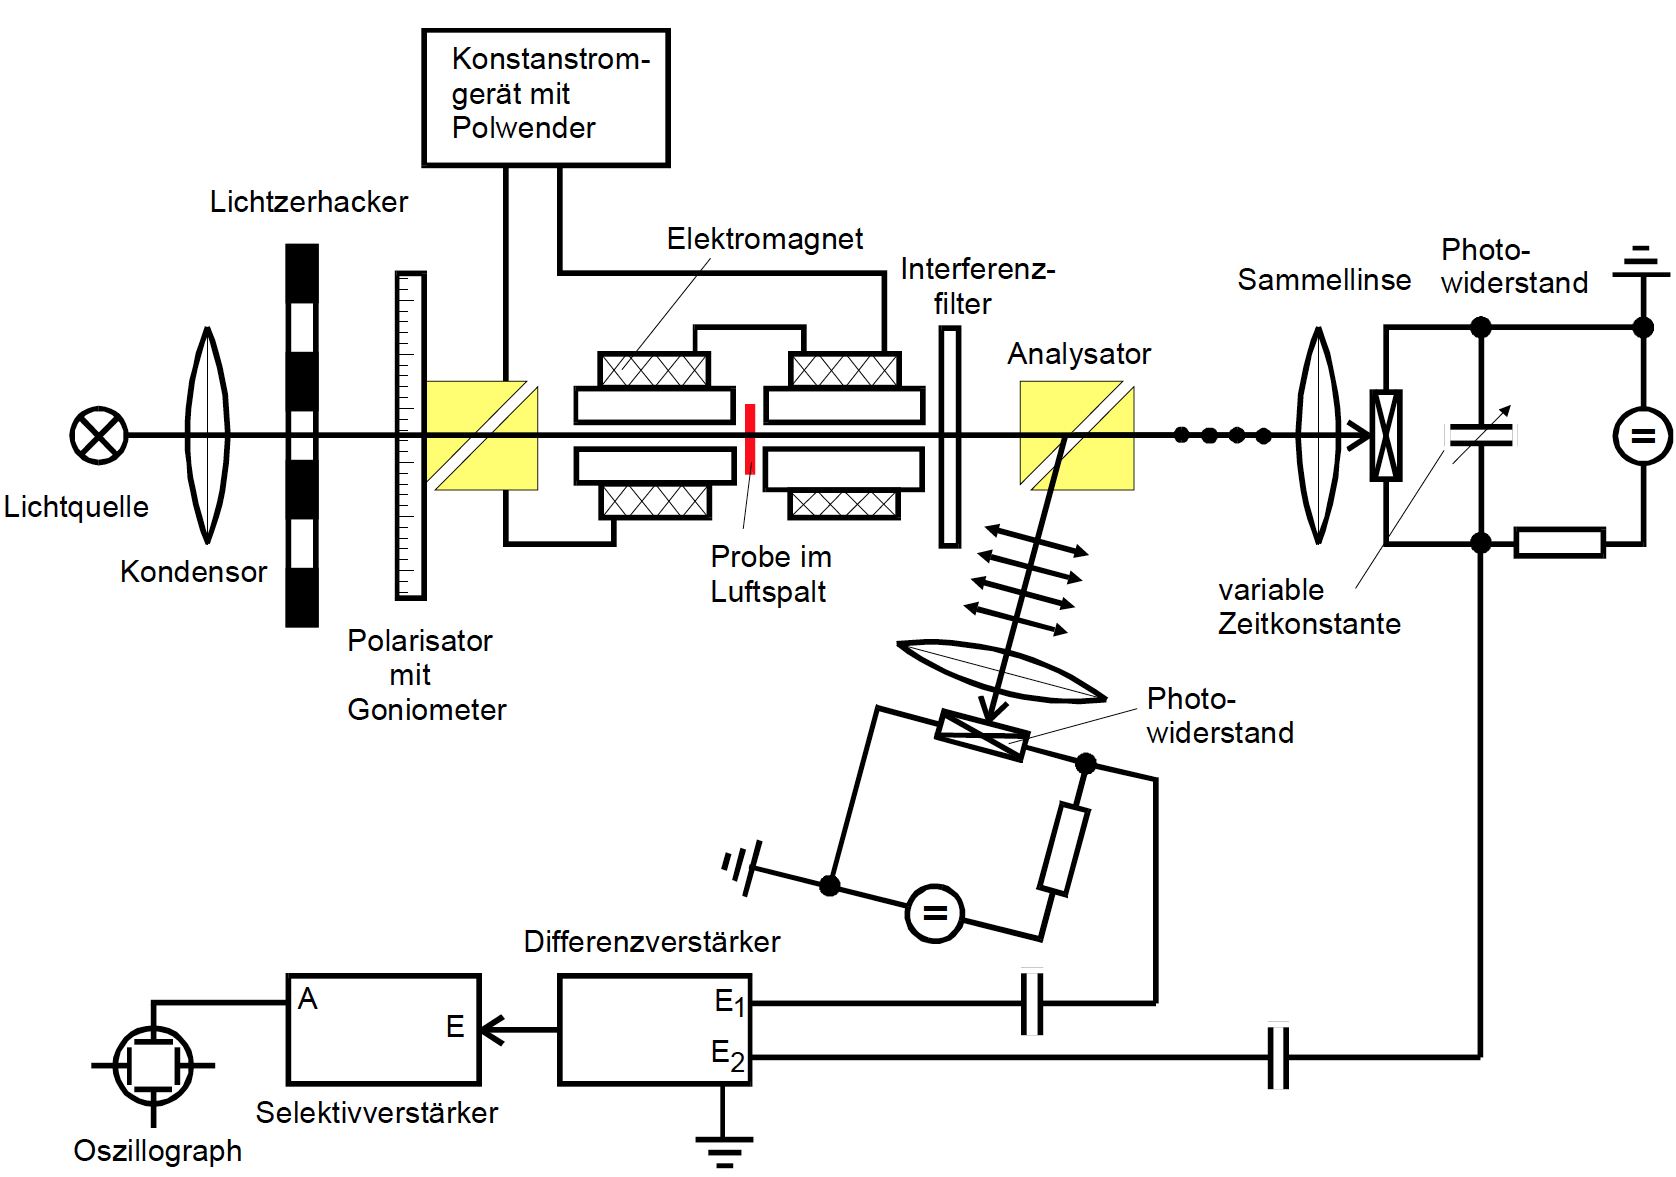
\includegraphics[width=0.9\textwidth]{aufbau.png}
    \caption{Schematischer Aufbau des Versuchs zur Messung der Faraday-Rotation mit Zweistrahlverfahren \cite{quelle03}.}
    \label{fig:aufbau}
\end{figure}
\FloatBarrier
\noindent
Eine Halogenlampe emittiert Licht im nahen Infrarot-Bereich. Dieses Licht durchläuft eine Sammellinse und einen 
Lichtzerhacker, der das einfallende Licht in Impulse zerhackt. Das Licht trifft dann auf das Glan-Thomson-Prisma aus
Kalkspat, wodurch es linear polarsiert wird. Hier ist außerdem ein Goniometer zur Messung der Winkelstellung integriert. 
Die scheibenförmige Probe befindet sich in der Symmetrieebene eines Elektromagneten, das mit einem Konstantstromgerät 
ein zeitlich konstantes Magnetfeld erzeugt. Hinter dem Magent befindet sich ein Interferenzfilter und ein zweites 
Glan-Thomson-Prisma, welches das einfallende Licht in zwei senktrecht zueinander polarisierte Strahlenbündel aufteilt,
die jeweils eine Sammellinse passieren und dann auf einen Photowiderstand aus Bleisulfid treffen, der die Lichtintensität misst. 
Die Photowiderstände sind an einen Differenzverstärker angeschlossen, der über einen Selektivverstärker mit
einem Oszilloskop verbunden ist. Die Ausgangsspannung des Differenzverstärkers ist proportional zur Differenz der 
Eingangsspannungen und verschwindet, sobal diese übereinstimmen, sodass das Oszilloskop als Nulldetektor genutzt wird.

\section{Durchführung}
Vor Beginn der Messung wird die Apparatur justiert. Außerdem wird mit der Probe und einem Interferenzfilter mit 
$1,06 \si{\micro \meter}$ überprüft, ob durch Drehen des Polarisators eine Signalamplitude von fast Null erreicht wird 
und ob nach eienr Drehung der Polarisators um etwa 90° ein weiteres Minimum aufritt.
Zuerst wird mit einer Hallsonde bei maximaler Stromstärke die magnetische Flussdichte $B(z)$ in Abhängigkeit vom 
Abstand $z$ gemessen. Zuerst wird dazu nach dem Maximum von $B(z)$ gesucht und dann um das Maximum herum mit Werten 
von $z = 100 \si{\milli\meter}$ bis $z = 127 \si{\milli\meter}$ die magnetische Flussdichte gemessen.
Dann wird mit drei GaAs-Proben, deren Eigenschaften in Tabelle \ref{tab:atab2} aufgeführt sind, und neun verschiedenen 
Interferenzfiltern von $1,06 \si{\micro \meter}$ bis $2,65 \si{\micro \meter}$ die Faraday-Rotation vermessen.
Dazu wird jeweils das Signal am Oszilloskop minimiert und die Winkeleinstellung am Goniometer abgelesen. Für jede Probe 
wird die Messung zweimal durchgeführt, wobei jeweils nach dem ersten Durchgang das Magnetfeld umgepolt wird.

%Auswertung
\section{Auswertung}
\subsection{Bestimmung der maximalen magnetischen Flussdichte}
In Tabelle \ref{tab:atab1} sind die gemessenen Werte für die magnetische Flussdichte dargestellt. 

\FloatBarrier
\begin{table}[h]
    \centering
    \caption{Messwerte der Magnetischen Flussdichte $B(z)$.}
    \label{tab:atab1}
    \begin{tabular}{s s | s s}
        \toprule
        {z/mm} & {B/mT} & {z/mm} & {B/mT} \\
        \midrule
        100 & 116 & 114 & 396 \\
        101 & 150 & 115 & 395 \\
        102 & 184 & 116 & 393 \\
        103 & 215 & 117 & 386 \\
        104 & 252 & 118 & 376 \\
        105 & 289 & 119 & 364 \\
        106 & 314 & 120 & 345 \\
        107 & 339 & 121 & 323 \\
        108 & 357 & 122 & 293 \\
        109 & 372 & 123 & 262 \\
        110 & 382 & 124 & 227 \\
        111 & 390 & 125 & 190 \\
        112 & 394 & 126 & 153 \\
        113 & 396 & 127 & 125 \\
        \bottomrule
    \end{tabular}
\end{table}
\FloatBarrier
\noindent

Diese werden in Abbildung \ref{fig:afig1} gegen $z$ aufgetragen und das Maximum bestimmt. 
Der Maximalwert der magnetischen Flussdichte entspricht dem Feld am Ort der Probe, somit wird für die nachfolgenen Rechnungen der Wert
\begin{equation}
	B = 396 \, \si{mT}
\end{equation}
verwendet.

\FloatBarrier
\begin{figure}[h]
    \centering
    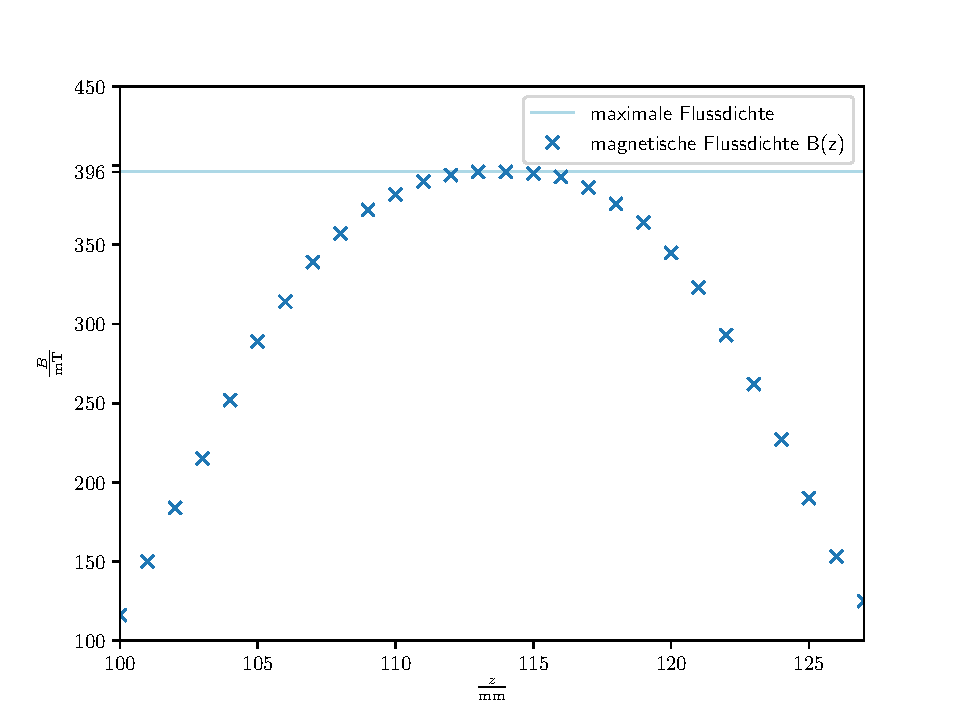
\includegraphics[width=\textwidth]{magnetfeld.pdf}
    \caption{Messwerte der Magnetische Flussdichte $B(z)$. Der Maximalwert liegt bei $B = 396\,\si{mT}$.}
    \label{fig:afig1}
\end{figure}
\FloatBarrier
\noindent


\subsection{Bestimmung der Rotationswinkel der Faraday Rotation}
Es werden drei verschiedene Proben von Galliumarsenid untersucht. Hierbei handelt es sich um eine undotierte und zwei n-dotierte Proben, deren Eigenschaften in Tabelle \ref{tab:atab2} zu finden sind.

\FloatBarrier
\begin{table}[h]
    \centering
    \caption{Eigenschaften der untersuchten Galliumarsenidproben.}
    \label{tab:atab2}
    \begin{tabular}{l c c c}
        \toprule
        {} & {Probe 1} & {Probe 2} & {Probe 3} \\
        \midrule
        Dotierung N/$cm^{-3}$ & - & $1,2 \cdot 10^{18}$ & $2,8 \cdot 10^{18}$ \\
        Dicke L/mm & 5,11 & 1,36 & 1,296 \\
        \bottomrule
    \end{tabular}
\end{table}
\FloatBarrier
\noindent


Die Messwerte der Drehwinkel sind in Tabelle \ref{tab:atab3} aufgelistet. Hierbei handelt es sich bei $\theta_1$ und $\theta_2$ je um die Winkel die bei unterschiedlich gepoltem Magnetfeld gemessen wurden.

\FloatBarrier
\begin{table}[h]
    \centering
    \caption{Messdaten für die Rotationswinkel für je zwei Polrichtungen des Magnetfeldes $B$, für 3 verschiedene Proben bei verschiedenen Wellenlängen.}
    \sisetup{table-format=2.1}
    \label{tab:atab3}
    \begin{tabular}{l c c c c c c}
        \toprule
        & \multicolumn{2}{c}{Probe 1} & \multicolumn{2}{c}{Probe 2} & \multicolumn{2}{c}{Probe 3} \\
        \cmidrule(lr){2-3}\cmidrule(lr){4-5}\cmidrule(lr){6-7}
        {$\lambda / \si{\micro\meter}$} & {$\theta_1$} & {$\theta_2$} & {$\theta_1$} & {$\theta_2$} & {$\theta_1$} & {$\theta_2$} \\
        \midrule

        1,06 & 143°50' & 167°00' & 148°20' & 158°00' & 150°10' & 159°30' \\
        1,29 & 148°00' & 164°00' & 150°00' & 157°20' & 150°35' & 157°20' \\
        1,45 & 148°20' & 160°15' & 146°35' & 154°50' & 150°10' & 159°00' \\
        1,72 & 151°00' & 160°00' & 149°40' & 156°15' & 149°20' & 161°10' \\
        1,96 & 157°30' & 164°40' & 250°35' & 161°50' & 154°25' & 164°30' \\
        2,156& 159°15' & 169°45' & 249°10' & 164°10' & 156°15' & 168°00' \\
        2,34 & 182°50' & 187°00' & 223°20' & 191°10' & 176°00' & 191°35' \\
        2,51 & 193°30' & 218°35' & 213°10' & 203°15' & 178°00' & 203°30' \\
        2,65 & 239°30' & 248°15' & 239°45' & 249°40' & 151°00' & 174°45' \\

        \bottomrule
    \end{tabular}
\end{table}
\FloatBarrier
\noindent

Für die nachfolgenden Rechnungen werden die Winkel, welche in Gradmaß angegeben sind, mittels der Formel
\begin{equation}
    1\, \symup{rad} = \frac{360°}{2\pi}
\end{equation}
in Bogenmaß umgerechnet. Hierbei ist zu beachten, dass die Gradmaß-Skala auf $60$ skaliert ist und somit
\begin{equation*}
    1' = 0.1\bar{6}°
\end{equation*}
entspricht. Der auf die Probenlänge normierte Rotationswinkel der Polarisationsebene errechnet sich dann mittels der Formel
\begin{equation}
    \theta = \frac{1}{2\, L}(\theta_2 - \theta_1) \qquad .
\end{equation}
Damit die Längeneinheiten die gleiche Einheit besitzen, wird $L$ hierzu in Mikrometer umgerechnet, da auch $\lambda$ diese Einheit hat.
In Tabelle \ref{tab:atab4} sind die umgerechneten und skalierten Werte des Rotationswinkels der einzelnen Proben zu finden. Diese Werte sind anschließend für jede der Proben gegen $\lambda^2$ 
aufgetragen, wie in den Abbildungen \ref{fig:afig2}, \ref{fig:afig3} und \ref{fig:afig4} dargestellt ist.

\FloatBarrier
\begin{table}[h]
    \centering
    \caption{Die gemessenen Rotationswinkel der drei Proben je auf die Probendicke skaliert.}
    \label{tab:atab4}
    \begin{tabular}{c c c}
        \toprule
        {$\theta_{\symup{Probe\,1}}/(10^{-5}\,\si{\micro\meter})$} & {$\theta_{\symup{Probe\,2}}/(10^{-5}\,\si{\micro\meter})$} & {$\theta_{\symup{Probe\,3}}/(10^{-5}\,\si{\micro\meter})$}\\
        \midrule
        4,03  & 6,20   &  6,28 \\
        2,73  & 4,70   &  4,55 \\
        2,03  & 5,29   &  5,95 \\
        1,54  & 4,22   &  7,97 \\
        1,22  & -56,94 &  6,79 \\
        1,79  & -54,54 &  7,91 \\
        0,71  & -20,64 &  8,42 \\
        4,28  & -6.37  &  4,94 \\
        1,49  & 6,37   &  10,83 \\
        \bottomrule 
    \end{tabular}
\end{table}
\FloatBarrier
\noindent
\FloatBarrier
\begin{figure}[h]
    \centering
    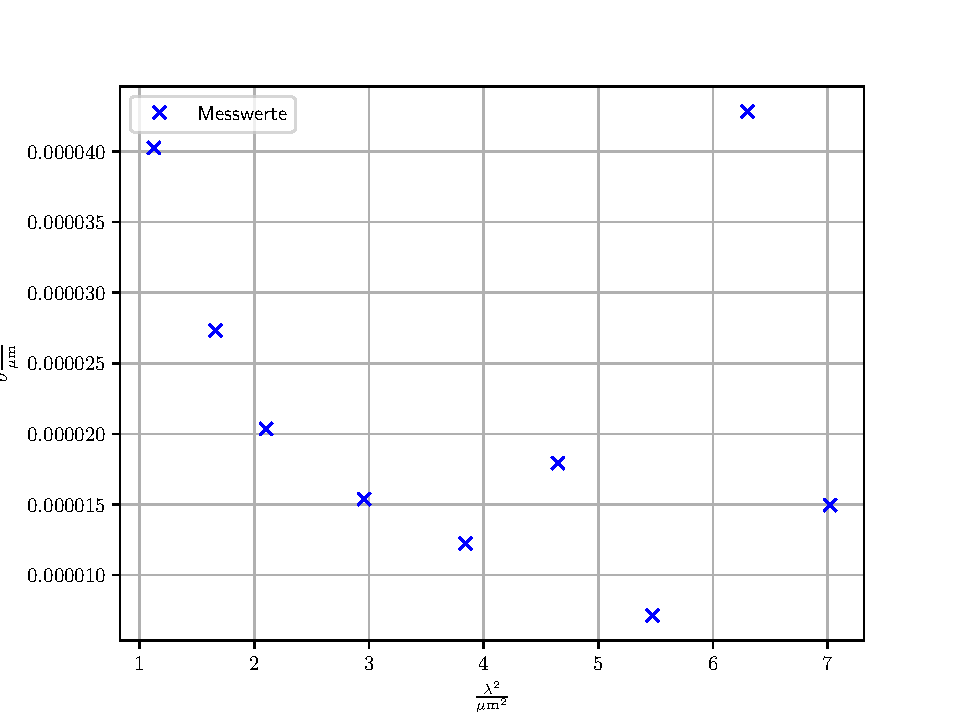
\includegraphics[width=1\textwidth]{Winkel_undotiert.pdf}
    \caption{Messwerte des Faraday-Rotationswinkels der Messung mit der reinen Galliumarsenidprobe (Probe 1). Der Rotationswinkel ist hierzu auf die Länge der Probe $L = 5110\, \si{\micro\meter}$ skaliert und gegen $\lambda ^2$ aufgetragen.}
    \label{fig:afig2}
\end{figure}
\FloatBarrier
\noindent

\noindent
\FloatBarrier
\begin{figure}[h]
    \centering
    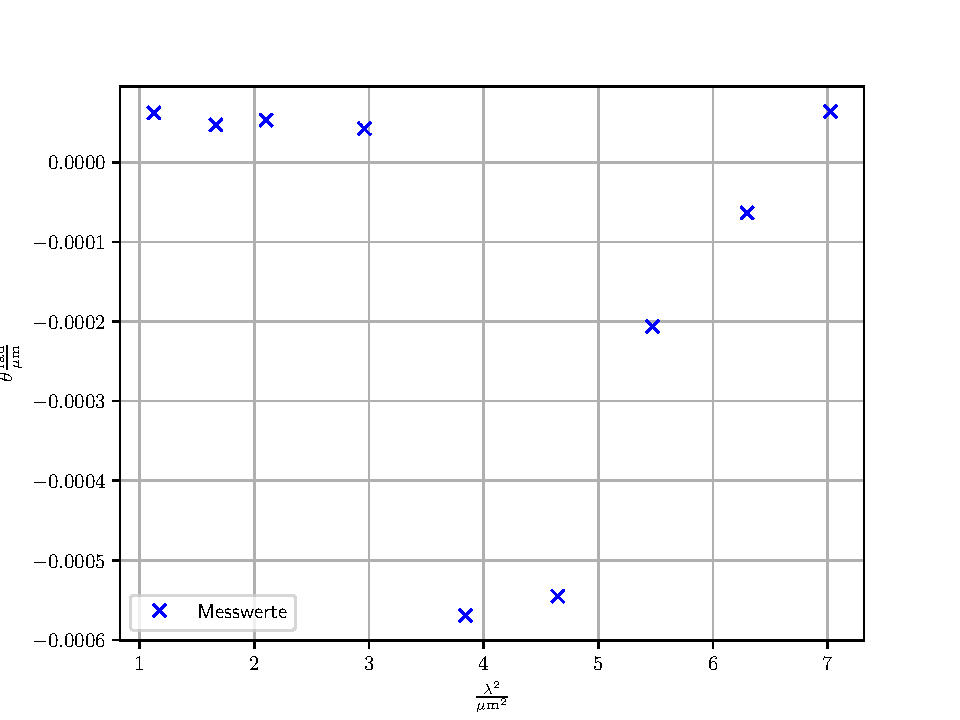
\includegraphics[width=1\textwidth]{Winkel_n-dotiert_1.pdf}
    \caption{Messwerte des Faraday-Rotationswinkels der Messung mit der dotierten Galliumarsenidprobe (Probe 2) mit einer Dotierungsdichte von $N=1,2\cdot 10^{18}\, \si{cm}^{-3}$. Der Rotationswinkel ist hierzu auf die Länge der Probe $L = 1360 \, \si{\micro\meter}$ skaliert und gegen $\lambda ^2$ aufgetragen.}
    \label{fig:afig3}
\end{figure}
\FloatBarrier
\noindent

\noindent
\FloatBarrier
\begin{figure}[h]
    \centering
    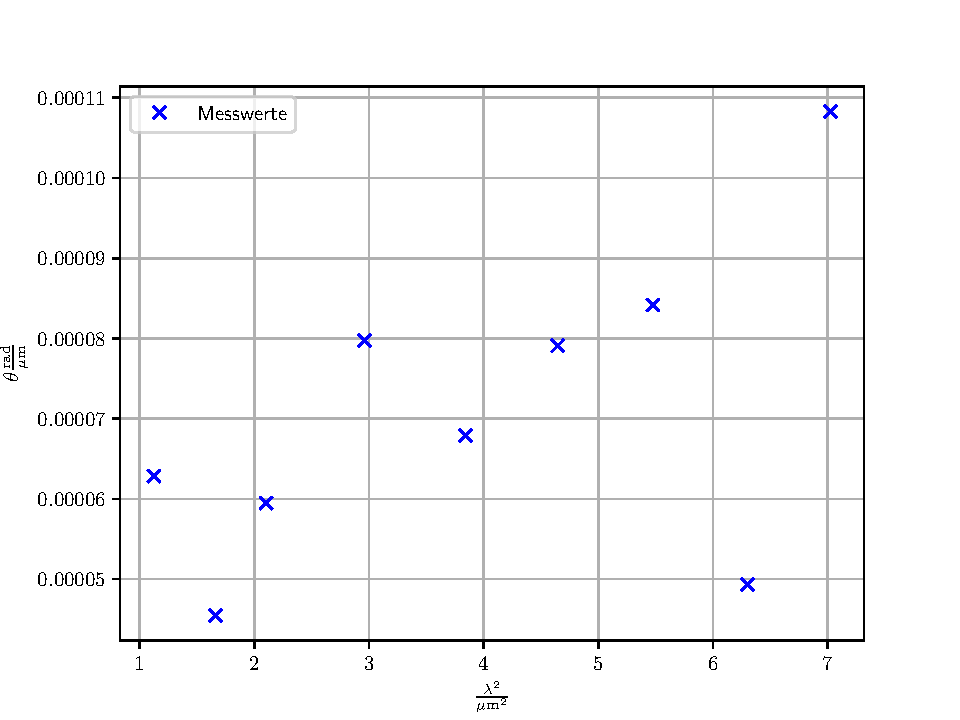
\includegraphics[width=1\textwidth]{Winkel_n-dotiert_2.pdf}
    \caption{Messwerte des Faraday-Rotationswinkels der Messung mit der dotierten Galliumarsenidprobe (Probe 3) mit einer Dotierungsdichte von $N=2,8\cdot 10^{18}\, \si{cm}^{-3}$. Der Rotationswinkel ist hierzu auf die Länge der Probe $L = 1296 \si{\micro\meter}$ skaliert und gegen $\lambda ^2$ aufgetragen.}
    \label{fig:afig4}
\end{figure}
\FloatBarrier
\noindent

\subsection{Bestimmung der effektiven Masse der Elektronen in Galliumarsenid}
Um die effektive Masse der Elektronen in dem Halbleiter zu bestimmen, wird der Rotationswinkel der durch die Leitungselektronen hervorgerufen wird gemäß
\begin{equation}
    \theta_{\symup{frei}} = |\theta_{\symup{undotiert}}-\theta_{\symup{dotiert}}| \label{eq:diff}
\end{equation}
berechnet und anschließend gegen $\lambda^2$ aufgetragen, wie in Abbildungen \ref{fig:afig5} und \ref{fig:afig6} für beide dotierte Proben zu sehen ist. 

\noindent
\FloatBarrier
\begin{figure}[h]
    \centering
    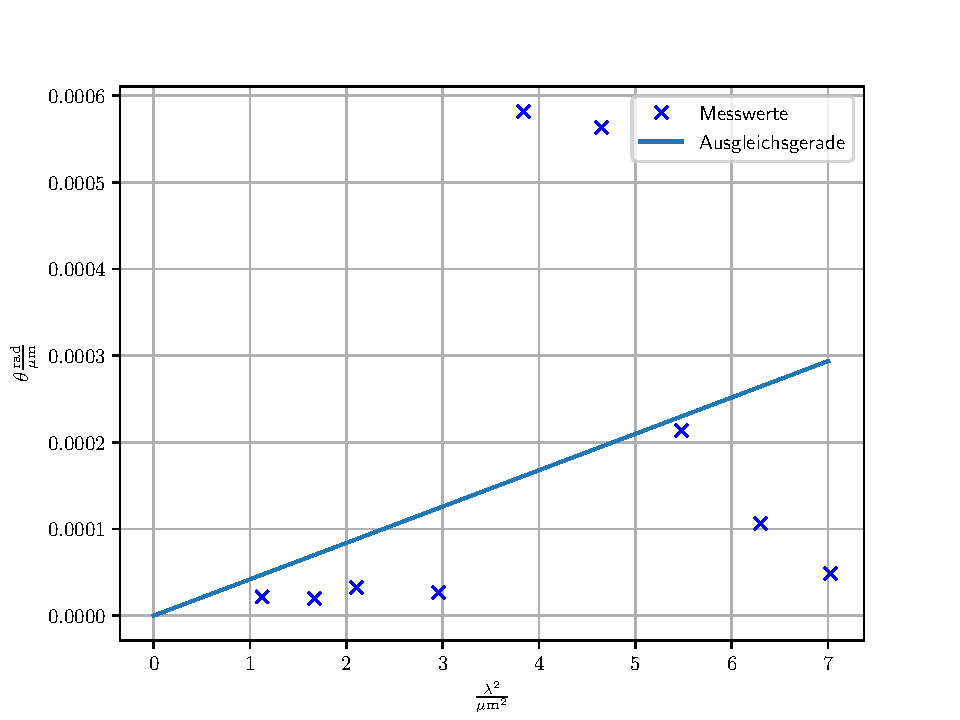
\includegraphics[width=1\textwidth]{Winkel_frei1.pdf}
    \caption{Der Rotationswinkel, welcher durch die Leitungselektronen hervorgerufen wird, aufgetragen gegen $\lambda^2$. Hierbei wurde $\theta_{\symup{frei}}$ aus dem Rotationswinkel der undotierten und der leicht dotierten Probe (Probe 2) gemäß \ref{eq:diff} berechnet.}
    \label{fig:afig5}
\end{figure}
\FloatBarrier
\noindent
\noindent
\FloatBarrier
\begin{figure}[h]
    \centering
    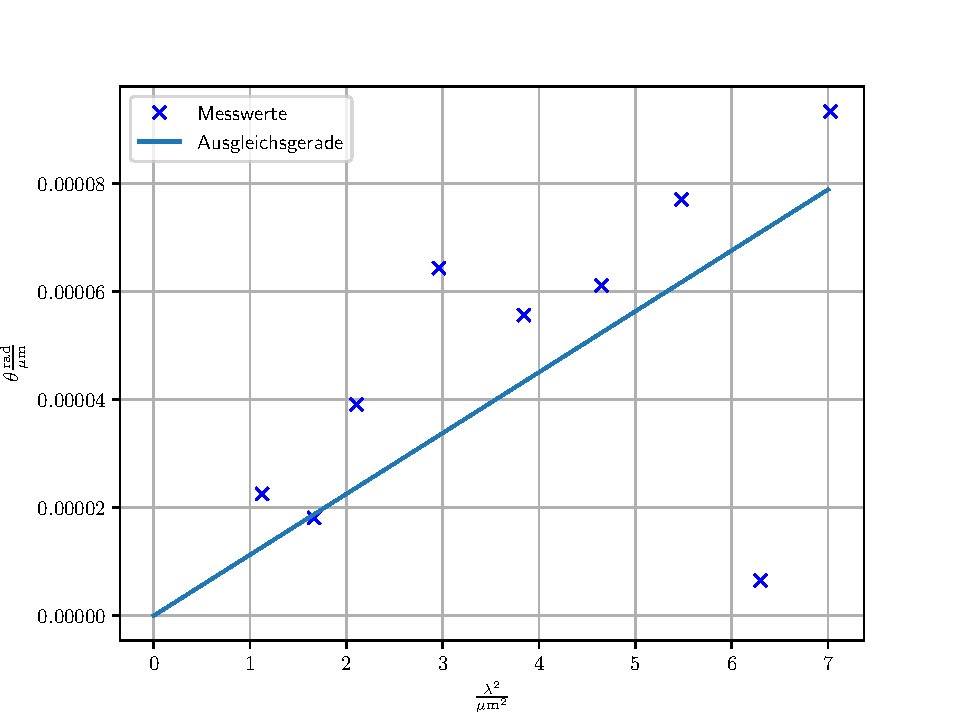
\includegraphics[width=1\textwidth]{Winkel_frei2.pdf}
    \caption{Der Rotationswinkel, welcher durch die Leitungselektronen hervorgerufen wird, aufgetragen gegen $\lambda^2$. Hierbei wird $\theta_{\symup{frei}}$ aus dem Rotationswinkel der undotierten und der stärker dotierten Probe (Probe 3) gemäß \ref{eq:diff} berechnet.}
    \label{fig:afig6}
\end{figure}
\FloatBarrier
\noindent

Zur Ermittlung des Proportionalitätsfaktors zwischen $\theta_{\symup{frei}}$ und
$\lambda^2$ wird eine Ausgleichrechnung
\begin{equation*}
    \theta_{\symup{frei}}(\lambda^2) = a\cdot \lambda ^2
\end{equation*}
durchgeführt.
Für diese ergeben sich die Proportianilitätsfaktoren
\begin{align*}
    a_1 &= (4,196 \pm 0,003)10^{-5}\, \si{\micro\meter}^{-3}\\
    a_2 &= (1,127 \pm 0,004)10^{-5}\, \si{\micro\meter}^{-3} \qquad .
\end{align*}

Der Zusammenhang zwischen dem Rotationswinkel $\theta_{\symup{frei}}$ und der Wellenlänge $\lambda$ ist gemäß Formel \ref{eq:Winkel}
gegeben, woraus sich mittels Koeffizientenvergleich für den Proportionalitätsfaktor der Zusammenhang \ref{eq:Prop} ergibt. Durch Umstellen der Gleichung \ref{eq:Prop} ergibt
sich der Ausdruck, mit welchem die effektive Masse berechnet werden kann
\begin{align}
   a &= \frac{e_0^3 \, N \, B}{8 \pi \epsilon_0 c^3 n (m^{*})^2}\\ \label{eq:Prop}
   \Leftrightarrow\qquad m &= \sqrt{\frac{e_0^3 \, N \, B}{8 \pi \epsilon_0 c^3 n a}} \, .
\end{align}
Zur Berechnung der effektiven Masse wird für den Brechungsindex der Literaturwert $n=3,857$ \cite{quelle04} verwendet. Somit folgen für die effektive Masse die beiden Werte
\begin{align*}
    m_1^{*} &= (0,02780 \pm 0.0001)\cdot m_e \\
    m_2^{*} &= (0.08192 \pm 0.0016)\cdot m_e \qquad .
\end{align*}

\section{Diskussion}
Wie erwartet ist bei der Messung der Kraftflussdichte des Magnetfeldes ein kleines Plateau beim Maximalwert zu erkennen. Somit konnte der Wert für das Feld am Ort der Probe leicht bestimmt werden.

Die gemessenen Werte der Rotationswinkel des undotierten Leiters in Abbildung \ref{fig:afig2} zeigen nicht den nach \ref{eq:Winkel2} erwarteten $\sim \frac{1}{\lambda^2}$ Verlauf. Dies lässt sich durch eventuelle Messfehler erklären.
Bei der Messung kam es bei einigen Wellenlängen zu dem Problem, dass der Nullabgleich sehr schwierig war. So kam es häufig bei kleineren Wellenlängen zu einer Übersteuerung des Selektivverstärkers. Ebenso war die Messung mit dem $1,72\,\si{\micro\meter}$
Plättchen besonders schwierig, da dieses einige Mängel aufwies. Es wirkte daher so, als würde mehr Licht durch das Plättchen durchkommen, als es eigentlich sollte, da häufig eine Übersteuerung bei minimaler Drehung des Glan-Thomson-Prismas auftrat.

Der Verlauf der Messwerte in Abbildung \ref{fig:afig3} und \ref{fig:afig4} kann vorerst nicht beurteilt werden, da hier der Einfluss aller Elektronen im Halbleiter eine Rolle spielt und somit keine genaue Aussage über die Abhängigkeit zur Wellenlänge $\lambda$ getroffen werden kann.
Jedoch sollte der Rotationswinkel des Faraday-Effekts, wenn der Einfluss der freien Elektronen isoliert wird, proportional zu $\lambda^2$ sein. Dieses Verhalten ist in den Abbildungen \ref{fig:afig5} und \ref{fig:afig6} nur begrenzt zu beobachten, wobei die Ergebnisse der stärker dotierten Probe
bis auf einen Ausreißer, annähernd den erwarteten linearen Verlauf zeigen.

Das Ergebnisse der Bestimmung der effektive Masse der Leitungselektronen in Galliumarsenid sidn
\begin{align*}
    m_1^{*} &= (0,02780 \pm 0.0010)\cdot m_e \\
    m_2^{*} &= (0.08192 \pm 0.0016)\cdot m_e \qquad .
\end{align*}
Verglichen mit dem Literaturwert für die effektive Masse der Leitungsbandelektronen im Halbleiter Galliumarsenid $m=0,063\, m_e$ \cite{quelle05} weist der erste Wert eine Abweichung von circa $55\%$ auf, während der zweite Wert
mit einer Abweichung von circa $30\%$ dem Literaturwert deutlich näher kommt. Der Mittelwert der beiden Ergebnisse $\bar{m} = (0,05486 \pm 0.0005)\cdot m_e$ weicht jedoch um nur $13\%$ vom Literaturwert ab. 

Zusammenfassend sind die Ergebnisse besser als der Verlauf der Messdaten zu Beginn vermuten lässt. Trotzdem sollte erwähnt werden, dass systematische Fehler dieses Experiment beinflusst haben. So war es zum Beispiel sehr schwierig, die Apparatur genau zu justieren, was sich bereits dadurch zeigte, dass die Winkel, bei dem der
Nullabgleich erreicht war, keinen $90°$-periodischen Verlauf zeigten, sondern eher $100°$-periodisch waren. Außerdem ist der Brechungsindex $n$, welche für die Berechnung der effektiven Masse $m^{*}$ benötigt wurde, ebenfalls abhängig von der Wellenlänge. Dieser wurde in diesem Experiment aber als konstant angenommen.

\nocite{wingate}
\nocite{*}
\printbibliography

\end{document}